Insertion Sort é um algoritmo de ordenação simples e intuitivo que constrói a saída final um item por vez. Ele é muito parecido com a forma como as pessoas ordenam cartas de baralho nas mãos. O algoritmo divide a entrada em duas partes: a sublista de itens já ordenados, que é construída a partida do zero, e a sublista de itens restantes a serem inseridos na lista ordenada. O algoritmo pega um item da segunda sublista em cada iteração e o insere na posição correta na primeira sublista.

\begin{figure}[htbp]
    \centering
    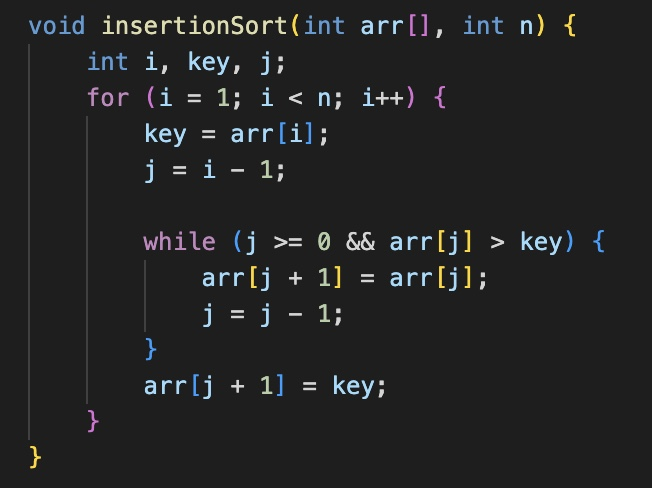
\includegraphics[width = 10cm]{Imagens/Insertion Sort/Imageminsert.jpg}
    \caption{Algoritmo Insertion Sort, criado pelo autor. }
    \label{fig:imagem_insert}
\end{figure}

\newpage
 Exemplo:\\
 Considere a seguinte entrada: 5, 2, 4, 6, 1, 3\\
 Saída esperada: 1, 2, 3, 4, 5, 6
\begin{figure}[htbp]
    \centering
    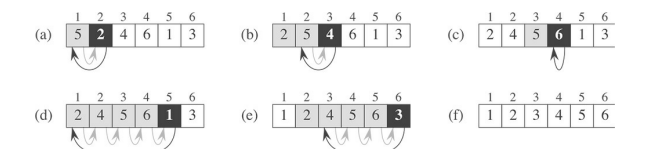
\includegraphics[width = 16cm]{Imagens/Insertion Sort/imagem1.png}
    \caption{Exemplo Insertion Sort retirado do livro Algoritmos: teoria e prática. }
    \label{grafico_insert}
\end{figure}

\cite{cormen2002}

O arranjo inicial a: [5, 2, 4, 6, 1, 3].
Primeira Iteração (índice 2, valor = 2):
comparamos 2 com 5 (à sua esquerda).
2 é menor, então trocamos.
Arranjo b: [2, 5, 4, 6, 1, 3]
Segunda Iteração (índice 3, valor = 4):
Comparamos 4 com 5.
4 é menor, então trocamos.
Arranjo c: [2, 4, 5, 6, 1, 3]
Terceira Iteração (índice 4, valor = 6):
Comparamos 6 com 5.
6 é maior, então não fazemos nada.
Arranjo d: [2, 4, 5, 6, 1, 3]
Quarta Iteração (índice 5, valor = 1):
Comparamos 1 com 6, 5, 4 e 2.
1 é menor que todos esses, então move-se para a primeira posição.
Arranjo e: [1, 2, 4, 5, 6, 3]
Quinta Iteração (índice 6, valor = 3):
Comparamos 3 com 6, 5, 4.
3 é menor que 6, 5 e 4, mas maior que 2.
Movemos 3 para a posição após 2.
Arranjo f: [1, 2, 3, 4, 5, 6]
Estado Final
Arranjo f: [1, 2, 3, 4, 5, 6].